\chapter{Browsers y Estado del Arte}
\label{chap4:EA}

\section{Arquitectura de Referencia del Browser y Patrones}
\label{chap3:ArqRefBrowandPatt}
%Referirme a los artículos que hayan realizado antes el trabajo
%usar: 2005-grosskurth-browser-refarch, preprint-grosskurth-browser-archevol, webpag3 (IE), reis2009isolating
%usar Larrondo 535061 (análisis de dominio del web browser)
% Godfrey2000 extrae architectura de software de Firefox

%Decir: "este trabajo es basado en la metodología de Fernandez \cite{Hashizume2014Reference} usando patrones en la construcción de la arquitectura de referencia"

\subsection{Método}
El primer paso para realizar el estado del arte con respecto a este punto fue realizar una búsqueda ordenada y a través de string de búsqueda dentro de web engines y librerías digitales conocidas. Se utilizaron las siguientes plataformas para buscar documentación al respecto:
\begin{itemize}
    \item Google, usando \textit{google dorks} para filtrar resultados
    \item Google Scholar, usando string de búsqueda y operadores booleanos para filtrar resultados.
    \item IEEE Xplore Digital Library, usando su buscador basado en comandos y utilizando operadores booleanos para filtrar (de buscó tanto en metadata como en el texto completo).
    \item Direct Science, CiteSeerX, Springer Link y otras librerías digitales. 
\end{itemize}

Para aquellos buscadores donde era posible usar operadores booleanos también se trató de filtrar el contenido para que pudiera mostrar resultados relacionados a: \textit{Browser} y \textit{Reference Architecture}. Sin embargo los resultados fueron bastante pobres. Desafortunadamente hasta la fecha no existe mucho trabajo relacionado a la construcción de una Arquitectura de Referencia para el Browser. Dado que la búsqueda no entregó muchos resultados, se procedió a hacer un \textit{forward snowballing} con el único paper que creemos entrega información similar a lo que se buscaba.

\subsection{Lo encontrado}
%larrondo
En Larrondo-Petrie et. al \cite{535061} se realiza un análisis orientado a objetos del dominio del web browser, con el fin de obtener un modelo de dominio, un modelo de objetos y un \textit{feature tree} que describiera la estructura y funcionalidad entregada comúnmente por los Web Browser. Sin embargo éste estudio está bastante lejos de lo que se quiere hacer en este trabajo, sin embargo sirve para obtener un transfondo de lo que sucede en el Web Browser, aún cuando la información esté muy desactualizada.

% preprint-grosskurth-browser-archevol y 2005-grosskurth-browser-refarch

En el trabajo de Grosskurth et al. \cite{2005-grosskurth-browser-refarch, preprint-grosskurth-browser-archevol} se llega a una arquitectura de referencia de muy alto nivel en base a dos navegadores open-source: Mozilla y Konqueror. En esta arquitectura se identifican los siguientes subcomponentes: Interfaz Usuaria, Persistencia de Datos, Browser Engine, Rendering Engine, Networking, Interprete de Javascript, XML Parser y Display Backend. Una vez obtenida la parte conceptual, se inició una evaluación de ésta al comparar las arquitecturas concretas de cada browser open-source, obtenidas por una herramientas de ingeniería inversa, para ver que tanto el modelo conceptual era cercano a la realidad; los browsers usados para validar fueron: Epiphany, Safari, Lynx, Mosaic y Firefox. Si bien la arquitectura entregada entrega bastante información a alto nivel, no desarrolla más que esa capa de abstracción. Además explica cada subsistema con los elementos que se deberían encontrar y para que son usados, por ejemplo explica que en el Rendering Engine es el encargado de mostrar lo parseado del HTML o XML de la página web e indica la relación de éste con el Browser Engine. 


%Godfrey2000
En el documento \cite{Godfrey2000} realizado en el año 2000, se describe la experiencia realizada al extender el rabajo del proyecto TAXFORM. Usando PBS, una herramienta de Ingeniería Inversa, se extrajo la arquitectura de software del Navegador Mozilla, con el objetivo de entender la estructuración de sus componentes. Si bien el trabajo ayuda a entender un poco la estructura detrás del navegador, este trabajo es muy antiguo y la versión más actual del navegador ha cambiado bastante. Además lamentablemente, el enfoque de este estudio no es intentar entender lo que hace cada subsistema, si no que es la implementación de la herramienta misma para obtener la arquitectura de software del browser seleccionado.

%Lwin2009 - Agent Based Web Browser
En \cite{Lwin2009} se propone un Browser llamado Anfel SOFT, donde gracias al uso de Inteligencia Artificial, crea agentes que permiten mejorar la experiencia del usuario. El trabajo asegura que el browser será capaz de aprender el comportamiento de navegación del usuario, y guiará al usuario en su navegación para que esta sea lo más efectiva posible. El paper obtiene los subsistemas que se pueden encontrar en un browser de la misma manera que lo realiza \cite{2005-grosskurth-browser-refarch}. Si bien la arquitectura que muestra refleja parte de lo visto en los 3 browsers escogidos en este estudio, no da detalles acerca de cada subsistema identificado. Además la arquitectura de Referencia que entrega es la misma vista en \cite{2005-grosskurth-browser-refarch, preprint-grosskurth-browser-archevol} y a pesar que identifica otros posibles componentes, no agrega nada nuevo.

Podemos ver en los trabajos ya mencionados, que la definición de Arquitectura de Referencia dista bastante de la definición dada por nosotros en el capítulo 2. En cada uno de ellos el trabajo ha sido a muy alto nivel y la descripción de los subcomponetes del sistema es mínima. Si bien explican las relaciones entre éstos, no dan un mayor entendimiento en como se comportan en ciertas situaciones. Desafortunadamente para esta memoria no existe mucha literatura sobre el desarrollo de una Arquitectura de Referencia del Browser, y de lo que hay el trabajo más actual es el realizado por \cite{Lwin2009} en el año 2009.


\section{Evolución y Seguridad en el Browser}
\label{chap3:EvoandSec}
%Usar referencias varga2013evolution, EvoBrowSecNSS, browSecPhish, browSecPrivSett, rowSecSEMBlock, silic2010security, barth2008security, reis2009browser, reis2009isolating, barth2009securing, barth2010protecting, Carlini12, liu2012chrome, utakrit2009review, barth2009secure, Accuvant11, Li12, Yu07, Zalewsk08, alcorn2014browser, sansInstInfoSec, 
% evolucion de la web: http://www.evolutionoftheweb.com/ (infografía)

En \cite{2005-grosskurth-browser-refarch} y \cite{preprint-grosskurth-browser-archevol} podemos notar que existe una mayor importancia en llegar a los componentes y las relaciones detrás del browser, y casi una nula mención de elementos de seguridad que permiten salvaguardar datos críticos o cómo protege al host de las amenazas. Podemos dar esta falta de conocimiento dado que en tales fehcas la cantidad de ataques de seguridad al Browser es mucho menos que en la actualidad %poner referencia.


\section{Navegadores Existentes}
\label{chap3:BrowExis}

    \subsection{Google Chrome y Google Chromium}
    \label{chap3:GC}
    La misión de Google es organizar la información del mundo y lograr que sea útil y accesible para todo el mundo. Esta gran empresa partió como un búscador y rápidamente llegó a ser dueño de la mayor parte de búsquedas del mercado. Tiene servicios de almacenamiento en la nube, correo electrónico, \textit{e-wallet} y otros más. Google ha sido responsable por la construcción del Navegador Web \textbf{Google Chrome} y \textit{Google Chromium}. En el 2008, Google liberó gran parte del código de Chrome bajo el proyecto de nombre Google Chromium, el cuál es open-source que permitiría a desarrolladores \textit{third-party}, estudiar el código fuente y ayudar en la implementación para las plataformas Linux y OS X. La diferencia entre Chrome y Chromium son: actualizaciones automáticas y Adobe Flash integrado (aunque éste último ya se está cambiando el uso por HTML5). En  \cite{EvolutionofWeb} se menciona que este Navegador ha sido el último que ha salido y se llevado una gran parte del mercado \cite{statBrow}.

    La arquitectura de Chrome o Chromium se basa principalmente en dos módulos: el Browser Kernel y el Rendering Engine, cómo se puede ver en la Figura \ref{fig:archG}.

    \begin{figure}[h!t]
        \centering
        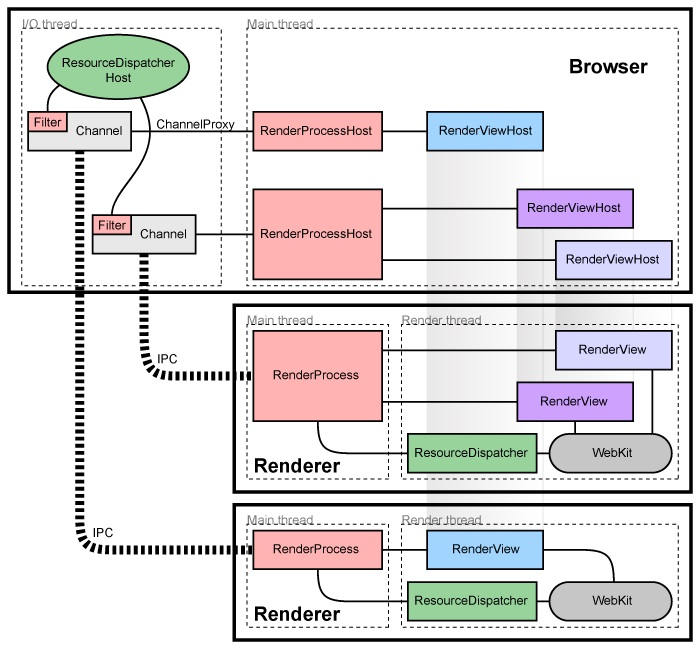
\includegraphics[scale=0.5]{figures/archGC.jpg}
        \caption{Architectura Multi procesos de Google Chrome. Fuente: \cite{multiProcGC}}
        \label{fig:archGC}
    \end{figure}

    \begin{figure}[h!t]
	    \centering
	    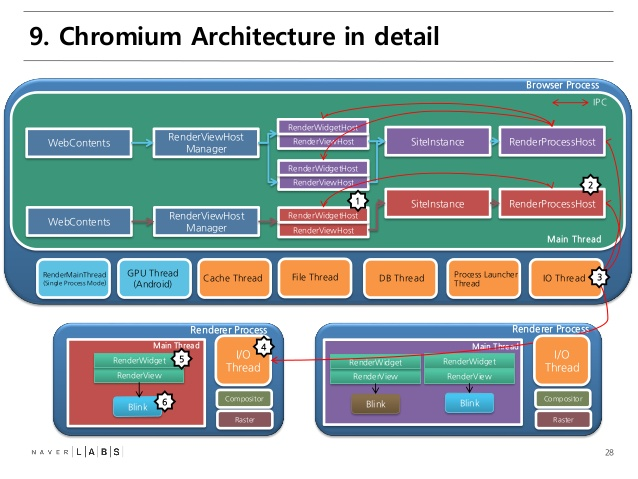
\includegraphics[scale=0.5]{figures/chromium-rendering-pipeline-28-638.jpg}
        \caption{Architectura de Chromium en detalle. Fuente: \cite{ChrRenderPipe}}
        \label{fig:archGC2}
    \end{figure}

    Én la documentación de Google Chromium \cite{multiProcGC}, que es base para Google Chrome, afirma que la arquitectura soporta para cada tab un proceso nuevo, de manera de hacer al Browser más robusto y modularizar el sistema para evitar ciertas amenazas de seguridad. El proceso principal es llamado \textit{Browser Process/Kernel/Engine} y se encarga de la \textit{User Interface}, manejo de las tabs y los procesos de los \textit{plug-in}. Cada tab es asociado a un Rendering Engine, éstos tienen restricciones de acceso (\textit{Sandoboxing}) a los demas y al sistema, lo que permite que exista una protección de la memoria y un control de acceso. En \cite{barth2008security} se explica que el objetivo principal de esta arquitectura es poder mitigar ataques muy severos sin tener que sacrificar la compatibilidad con los sitios web ya existentes. Para lograr el objetivo Google ha ganado muchas lecciones de cómo realizar esto \cite{reis2009browser}, pues explican que un gran desafío en la seguridad es proteger a los usuarios de los atacantes que se aprovechan de las vulnerabilidades y debilidades de los clientes web-browsers. En su arquitectura modular se puede ver que se intenta proveer una seguridad que evita afectar la compatibilidad con otros sitios. La arquitectura comentada se basa en dos decisiones de diseño: La arquitectura depende en el Rendering Engine para aquellos componentes de alto riesgo como JavaScript, el parser de HTML y la creación de DOM para hacer cumplir SOP; al estar rodeados por un Sandboxing hace que el Rendering Engine se comporte como una caja negra. 


    Google Chrome expone en \cite{reis2009browser} que existen ciertas lecciones que han ido utilizando para mejorar la calidad de su browser. Estas son:

    \begin{itemize}
    	\item Reducción de las vulnerabilidades de seguridad, se basa en la aislación de ciertos componentes y la reducción de privilegios de ciertas tareas en el browser. La aislación lo lograron con la creación del Rendering Engine y el Browser Kernel, que tienen como objetivo proteger la data del sistema de archivos. Si bien esto puede no entregar muchos beneficios a una aplicación web, si lo hace en el usuario del browser.
    	\item Reducir la ventana de vulnerabilidades, la actualización del browser se hace cada cierto tiempo de forma automática para así cubrir las vulnerabilidades que van apareciendo.
    	\item Reducción de la frecuencia de exposición, Google trabaja con StopBadware.org para entregar una mayor seguridad al descubrir nuevos tipos de ataques y vulnerabilidades relacionadas con el browser.
    \end{itemize}

    \subsubsection{Browser Engine/Process}

    \subsubsection{Renderering Engine/Process - Blink}
     \label{chap2:Blink}
     Es el \textit{Rendering Engine} usado por Google Chrome/Chromium y es el \textit{forking} del trabajo original llamado Webkit. Su objetivo principal es soportar la architectura de multi-procesos que posee el navegador y al mismo tiempo poder reducir el nivel de complejidad.


    %     \begin{figure}[h!t]
    %     \begin{center}
    %         \includegraphics[scale=0.5]{figures/in_process_plugins.png}
    %       %\caption{Representación conceptual de una Nube con Eucalyptus. La especificación de las partes y su explicación se ve en \ref{sec:chap2.4.2}. Fuente \cite{EucalyptusOverview}}
    %       \label{fig:archG}
    %     \end{center}
    % \end{figure}


    % \begin{figure}[h!t]
    %     \begin{center}
    %         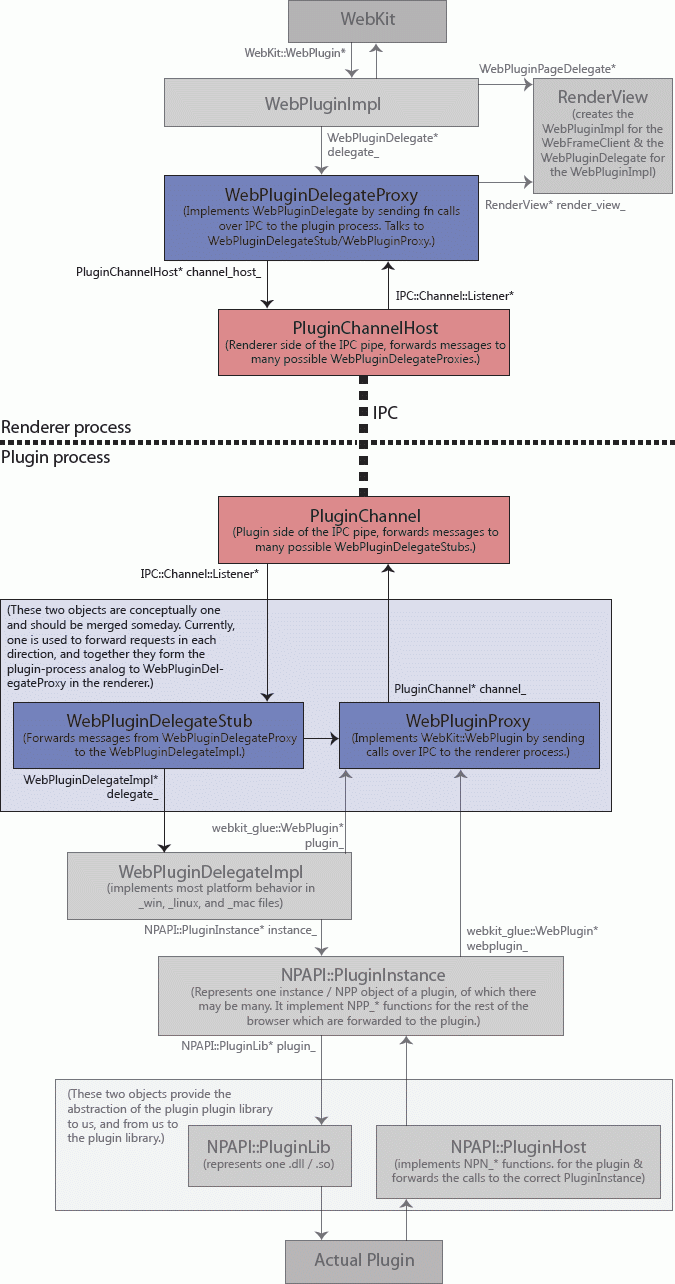
\includegraphics[scale=0.5]{figures/out_of_process_plugins.png}
    %       %\caption{Representación conceptual de una Nube con Eucalyptus. La especificación de las partes y su explicación se ve en \ref{sec:chap2.4.2}. Fuente \cite{EucalyptusOverview}}
    %       \label{fig:archG}
    %     \end{center}
    % \end{figure}

    % \begin{figure}[h!t]
    %     \begin{center}
    %         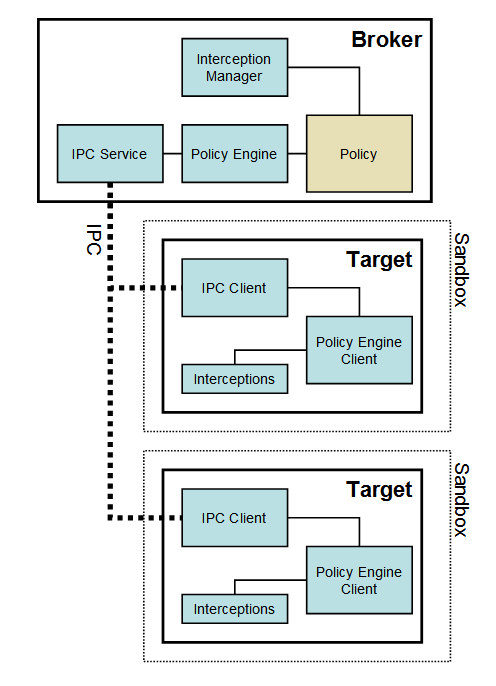
\includegraphics[scale=0.5]{figures/sbox_top_diagram.png}
    %       %\caption{Representación conceptual de una Nube con Eucalyptus. La especificación de las partes y su explicación se ve en \ref{sec:chap2.4.2}. Fuente \cite{EucalyptusOverview}}
    %       \label{fig:archG}
    %     \end{center}
    % \end{figure}

        \subsubsection{Extensions}

        \subsubsection{Plugins}

        \subsubsection{Aislación - Isolation}
            siteinstance-per-process, aunque están tratando de mejorarlo a site-per-process \cite{GoogleChromeIsolation}
        \subsubsection{Sandbox}
            -Sandbox, propia implementación + el del sistema operativo – políticas
            -restringuir el ingreso al file system



    \subsection{Internet Explorer}
    \label{chap3:IE}
    Internet Explorer es el navegador grafico predeterminado por Microsoft y que su primera versión 1.0 fue realizada en 1995. IE es una derivación de Spyglass Mosaic desarrolado por la NCSA (National Center for Supercomputing Applications). En primera instancia fue un navegador que podría ser obtebido si era comprado como complemento de \textit{Microsoft Plus!} o mediante la versión \textit{OEM} de Windows 95. Desde la tercera versión de IE, en 1996, que esta se lanzó de forma gratuita.
            
    La arquitectura de este navegador es modular y permite al desarrollador por utilizar los recursos para crear diferentes funcionalidades, ejemplo de esto son: toolbars, Microsoft Active X controls, etc. En la Figura \ref{fig:archIE} \cite{IEArch} se puede ver los principales componentes de la architectura del browser mencionado. IE utiliza \textit{COM} o \textit{Component Object Model} una interfaz binaria standard para componentes de software introducida por Microsoft en 1993 y que permite una comunicación entre procesos/componentes de software provenientes de la familia de software de Microsoft. \textit{COM} es similar a otras tecnologías de interfaz de componentes de software ( Component Software Interface Technologies) cómo CORBA y Java Beans. El uso de \textit{COM} gobierna la forma la interacción de los componentes que se comunicann y permite que haya un reuso y extensibilidad de estos.
            
	\begin{figure}[h!t]
	    \centering
		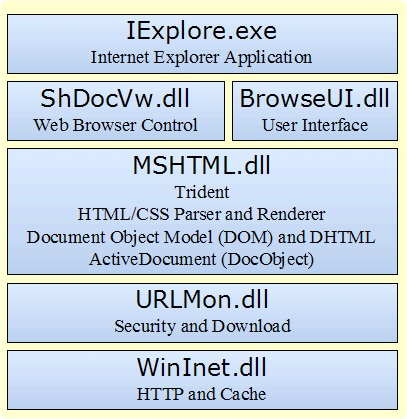
\includegraphics[scale=0.65]{figures/IEArch.jpg}
		\caption{Arquitectura de Internet Explorer. Fuente: \cite{IEArchImg}}
		\label{fig:archIE}
    \end{figure}

    \begin{figure}[h!t]
        \centering
        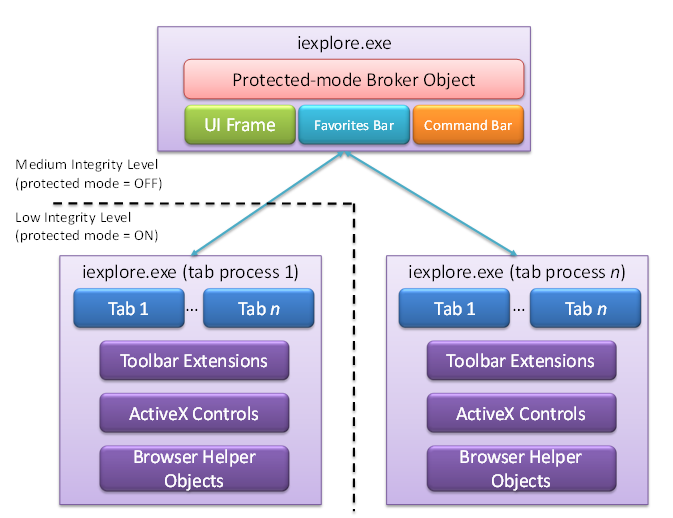
\includegraphics[scale=0.5]{figures/11_IE8andLooselyCoupledIELCIE_2.png}
        \caption{Arquitectura de Internet Explorer más detallada. Fuente: \cite{IE8LCIE}}
        \label{fig:archIE2}
    \end{figure}

        \subsubsection{Frame Process}

   
        \subsubsection{Rendering Engine}   
        \label{chap2:Trident}
        O también llamado MSHTML, es un rendering engine privativo, sin embargo es posible usarlo al usar librería de Windows \textbf{mshtml.dll}. Según \cite{Crowley2010} es un objeto OLE (Object Linking and Embedding) Active Document que representa el \textit{layout} de Internet Explorer y permite mostrar graficamente las páginas por medio del \textit{display} del host. Dentro de éste se manejan las Extenciones, el \textit{engine} de Javascript y la librería que contiene la API para tareas de \textit{networking}, además de proveer una capa de seguridad y manejar las descargas de archivos.

        \subsubsection{HBO}

        \subsubsection{Plugins}

        \subsubsection{Aislación}

        \subsubsection{Sandbox}

    \subsection{Firefox}
    \label{chap3:Firefox}

    Firefox fue creado a partir del navegador \textit{Netscape} en 1998, actualmente la fundación Mozilla ha sido la que la ha mantenido, generando varias modificaciones desde su nacimiento. Las metas de diseño que Mozilla desee en el navegador son:
    \begin{itemize}
        \item Renderizado rápido de las páginas web.
        \item Fuerte apoyo a los estandares web como la W3C.
        \item Interoperabilidad en las diversas plataformas.
    \end{itemize}

    \subsubsection{Firefox Mono-proceso}
        \begin{figure}[h!t]
    		\centering
        	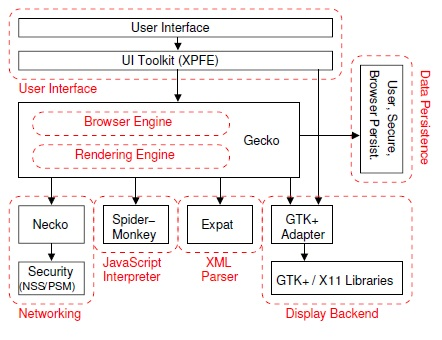
\includegraphics[scale=0.8]{figures/archMoz.jpg}
            %\caption{Representación conceptual de una Nube con Eucalyptus. La especificación de las partes y su explicación se ve en \ref{sec:chap2.4.2}. Fuente \cite{EucalyptusOverview}}
            \label{fig:archM}
        \end{figure}
                
        La arquitectura de este browser puede ser vista en la Figura \ref{fig:archM} donde se pueden observar los siguientes componentes:
                \begin{itemize}
                    \item La interfaz de usuario, puede ser reutilizada para otras aplicaciones.
                    \item La persistencia de los datos, tanto de bookmarks como de data de bajo nivel como el \textit{cache}.
                    \item EL \textit{Rendering Engine}, permite el renderizado de documentos HTML/XML aún cuando estos estén mal formados. Este Engine es capaz de renderizar la interfaz de la aplicación multi-plataforma.
                \end{itemize}
        La arquitectura de Mozilla se distingue de las demás en que la visualización especificada por la plataforma y la librería de \textit{widgets} son usados directamente en el navegador, lo que minimiza el costo necesario para soportar diferentes plataformas.

        Gecko es un motor de renderizado \textit{Open Source} que utiliza Firefox, escrito en C++, creado en un comienzo por Netscape, predecesor de Mozilla Foundation/Corporation. La función de este componente en Firefox (y otros browsers que lo integran) es leer el \textit{web content} de tipo HTML, CSS, XUL (para renderizar \textit{User Interface}) y Javascript, y mostrarlo al usuario en un formato gráfico. Tiene un gran rendiemiento al transformar a formato gráfico una página con lenguaje de marcado ya que soporta multithreading en el parser de HTML. Gecko fue diseñado para soportar \textit{Open Internet Standards} y por ende sigue al pie de la letra todas las especificaciones de HTML 4, CCS 1 y 2, DOM, XML y Javascript. Los componentes de Gecko incluyen:
            \begin{itemize}
                \item Parser de Documentos (HTML y XML).
                \item \textit{Layout Engine} con un modelo de contenido; ésta es la información que el display del host mostrará al usuario.
                \item Sistema de estilos.
                \item Motor de Javascript. En el caso de Gecko éste se llama \textbf{SpiderMonkey} que está escrito en C/C++.
                \item Librería de imágenes.
                \item Librería de \textit{Networking}.
                \item Renderizado gráfico específico a la plataforma y widget de acuerdo al sistema operativo.
                \item Librerías de Seguridad.
                \item librería de preferencias de usuario, entre otros más.
            \end{itemize}

        \begin{figure}[h!t]
            \centering
            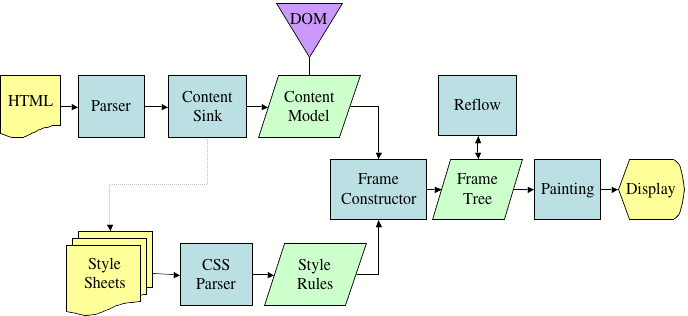
\includegraphics[width=0.8\textwidth]{figures/Gecko_Overview_9.png}
            \caption{Gecko Rendering Engine. Fuente: \cite{gecko}}
            \label{fig:Gecko}
        \end{figure}

        
    \subsubsection{Firefox Multi-proceso (Electrolysis)} 

            

\section{Sumario}
\label{chap3:Summ}



% \subsection{Rendering Engines}
% \label{chap2:RenderingE}
% Responsable de converitir la página web, en HTML o XML, a un formato visible cómodo para el usuario en la pantalla del host. La combinación de HTML, CSS y media (imagenes, videos, etc.) permiten entregar una experiencia gráfica al usuario con la que interactuará. Existen browser que no usan gráficos y solo se basan en mostrar texto, ejemplos de estos navegadores son: W3M y Lynx. Los \textit{Rendering Engines} más usados son: Webkit (Safari), Blink (Google Chrome/Chromium), Trident (Internet Explorer) y Gecko (Firefox).

%     \subsubsection{Trident}
%     
%     







